\section*{Exercise 6}

\subsection*{Exercise 6.1}
To see the problems of rejection sampling, consider the following variation of the previous example:

\begin{lstlisting}
(define baserate 0.1)
(define (take-sample)
  (rejection-sampler
   (define A (if (flip baserate) 1 0))
   (define B (if (flip baserate) 1 0))
   (define C (if (flip baserate) 1 0))
   (define D (+ A B C))
   (observe/fail (>= D 2))
   A))
\end{lstlisting}

Try to see what happens when you lower the basesate. What happens if we set it to 0.01? And to 0.001?

\paragraph{Solution}
In order to assess the differences between different baserates, it has been developed a program which generates $100$ samples for each
baserate and computes the histogram of the results. The code is shown below:
\begin{lstlisting}
(define (model baserate)
  (define (take-sample)
    (rejection-sampler
     (define A (if (flip baserate) 1 0))
     (define B (if (flip baserate) 1 0))
     (define C (if (flip baserate) 1 0))
     (define D (+ A B C))
     (observe/fail (>= D 2))
     A))
  (take-sample))

; experiment with baserate = 0.1
(hist (repeat (model 0.1) 1000))

; experiment with baserate = 0.01
(hist (repeat (model 0.01) 1000))

; experiment with baserate = 0.001
(hist (repeat (model 0.001) 1000))
\end{lstlisting}

The procedure \texttt{model} has been developed in order to be able to pass the baserate as parameter of the procedure. So the 
procedure \texttt{model} is a wrapper for the procedure \texttt{take-sample}. In this way it is possible to call the procedure 
\texttt{take-sample} with different baserates by passsing a different parameter to the procedure \texttt{model}.
Then three different experiments are run: \textit{(i)} The baserate is set to $0.1$; \textit{(ii)} The baserate is set to $0.01$;
\textit{(iii)} The baserate is set to $0.001$.
By observing the histograms of the results of the different experiments we can conclude that the computed probability is more or less
the same in all three cases, but the main difference is that the time of execution is completely different.
In particular the first example (i.e. $baserate = 0.1$) is faster than the other two cases. 
Furthermore the case with $baserate = 0.01$ takes much less time that the third case.

This behaviour is due to the probability to get at least two successful results, in particular the lower is the baserate the lower
is the probability that the procedure \texttt{flip} returns \texttt{\#t} so the lower is the probability that \texttt{A}, \texttt{B}
and \texttt{C} are equal to one.
Since we are approximating the posterior probability $ P(A | D >= 2) $ by rejection sampling, all the samples which do not agree with
the evidence (i.e. $D = 2$) are discarded. When the baserate is high the probability of getting $ D >= 2 $ increases, so it is
less likely that the sample is discarded, instead if the baserate is low, then the probability to discard a sample increases
because it is more probable that the variables \texttt{A}, \texttt{B} and \texttt{C} are equal to zero.

The results of the approximated probabilities are shown in Figure~\ref{fig:baserate-1}, Figure~\ref{fig:baserate-01} and
Figure~\ref{fig:baserate-001}. It is possible to observe that $ P(A = 0 | D >= 2) \approx 1/3 $ and 
$ P(A = 0 | D >= 2) \approx 2/3 $.

\begin{figure}[ht!]
  \centering
  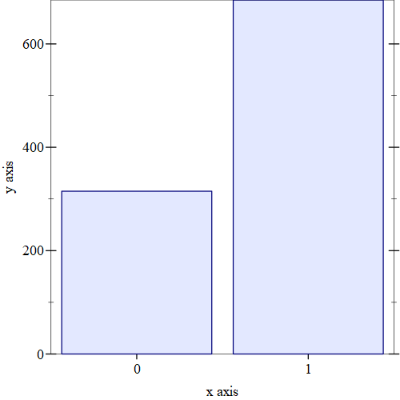
\includegraphics[width=7cm]{images/6.1.png}
  \caption{
    Approximate posterior probability $ P(A | D >= 2) $ with $baserate = 0.1 $
  }
  \label{fig:baserate-1}
\end{figure}
\begin{figure}[ht!]
  \centering
  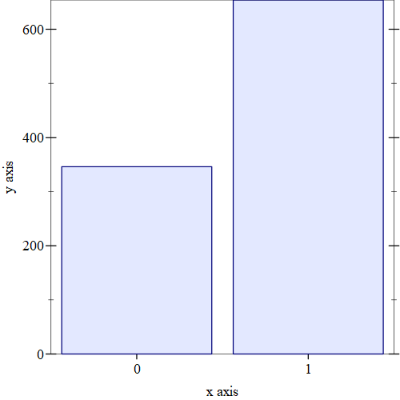
\includegraphics[width=7cm]{images/6.2.png}
  \caption{
    Approximate posterior probability $ P(A | D >= 2) $ with $baserate = 0.01 $
  }
  \label{fig:baserate-01}
\end{figure}
\begin{figure}[ht!]
  \centering
  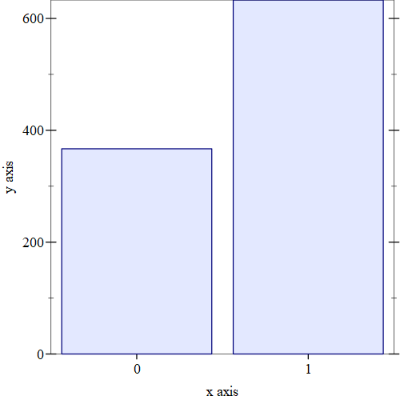
\includegraphics[width=7cm]{images/6.3.png}
  \caption{
    Approximate posterior probability $ P(A | D >= 2) $ with $baserate = 0.001 $
  }
  \label{fig:baserate-001}
\end{figure}